%نام و نام خانوادگی:
%شماره دانشجویی: 
\مسئله{پارسر \lr{LALR(1)}}

\پاسخ{ }
\\
الف) عکس دیاگرام در زیر قرار داده شده است:
\graphicspath{{./images/}}
\begin{center}
	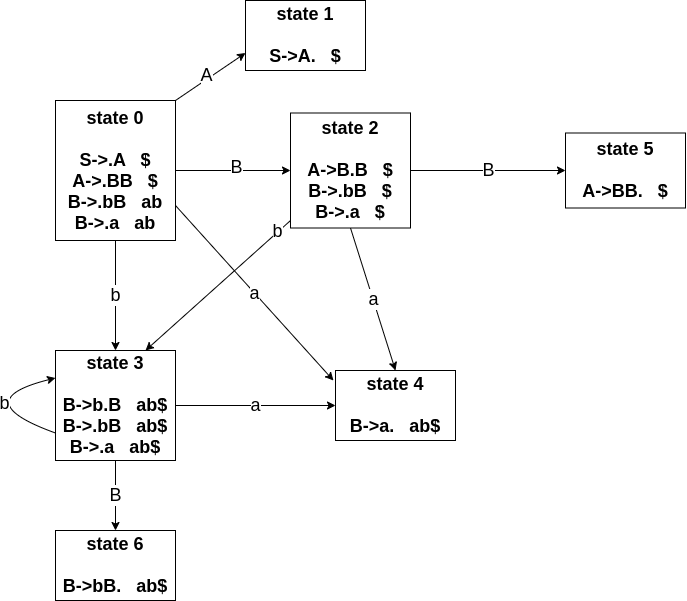
\includegraphics[scale=0.7]{compiler_hw2_q9.png}
\end{center}
عکس جدول در زیر قرار داده شده است:
\include{{./images}}
\begin{center}
	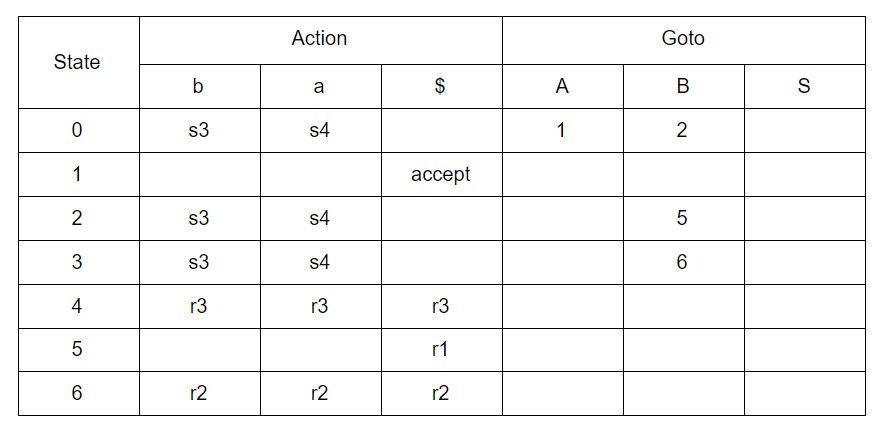
\includegraphics[scale=0.9]{compiler_hw2_q9_table.png}
\end{center}
ب) درخت پارس $babba$ را در پایین نوشته‌ایم: (دقت شود که حروفی که بین دو | می‌آیند در مرحله بعدی قرار است با هم، به کمک قاعده تولید reduce شوند)
\begin{latin}
	b
	\\
	b a
	\\
	b |a|
	\\
	b B
	\\
	|b B|
	\\
	B
	\\
	B b
	\\
	B b b
	\\
	B b b a
	\\
	B b b |a|
	\\
	B b b B
	\\
	B b |b B|
	\\
	B b B
	\\
	B |b B|
	\\
	B B
	\\
	|B B|
	\\
	A
\end{latin}
در نهایت درخت پارس رشته به صورت زیر می‌شود: (به دو صورت عکس و کتابخانه خود latex نمایش داده شده است)
\begin{center}
	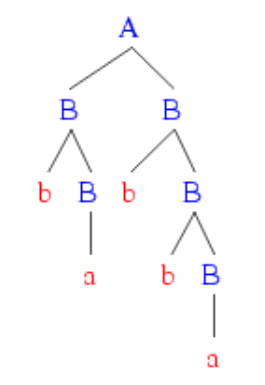
\includegraphics{babba.png}
\end{center}
\begin {center}
\begin {tikzpicture}[-latex ,auto ,node distance =2 cm and 1cm ,on grid ,
semithick ,
state/.style ={ circle ,top color =white , bottom color = white ,
	draw,white , text=black , minimum width =1 cm}]
\node[state] (0){$A$};
\node[state] (1) [below left=of 0] {$B$};
\node[state] (2) [below right=of 0] {$B$};
\node[state] (3) [below left=of 1] {\lr{$b$}};
\node[state] (4) [below =of 1] {\lr{$B$}};
\node[state] (5) [below =of 2] {\lr{$b$}};
\node[state] (6) [below right=of 2] {$B$};
\node[state] (7) [below =of 4] {\lr{$a$}};
\node[state] (8) [below left=of 6] {\lr{$b$}};
\node[state] (9) [below right =of 6] {\lr{$B$}};
\node[state] (10) [below  =of 9] {\lr{$a$}};



\path (0) edge [] node[left] {} (1);
\path (0) edge [] node[] {} (2);
\path (1) edge [] node[] {} (3);
\path (1) edge [] node[] {} (4);
\path (2) edge [] node[] {} (5);
\path (2) edge [] node[] {} (6);
\path (4) edge [] node[] {} (7);
\path (6) edge [] node[] {} (8);
\path (6) edge [] node[] {} (9);
\path (9) edge [] node[] {} (10);


\end{tikzpicture}
\end{center}








